\documentclass{article}
\usepackage{tikz}
\usepackage{tkz-euclide}
\definecolor{darkgreen}{RGB}{0,192,0}
\title{Cartesian closed categories and the price of eggs}
\author{Jane Doe}
\date{September 1994}
\begin{document}

	\begin{figure}
		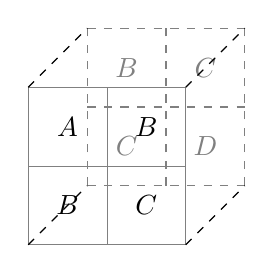
\begin{tikzpicture}
			\draw[step=1cm,gray,very thin] (0,0,0) grid (2,-2,0);
			\draw (0.5,-0.5) node {$A$};
			\draw (1.5,-0.5) node {$B$};
			\draw (0.5,-1.5) node {$B$};
			\draw (1.5,-1.5) node {$C$};

			\begin{scope}[shift={(0.75,0.75,0)}]
				\draw[step=1cm,gray,dashed] (0,0,0) grid (2,-2,0);
				\draw[gray] (0.5,-0.5) node {$B$};
				\draw[gray] (1.5,-0.5) node {$C$};
				\draw[gray] (0.5,-1.5) node {$C$};
				\draw[gray] (1.5,-1.5) node {$D$};
			\end{scope}

			\draw[dashed] (0,0,0) -- (0.75, 0.75,0);
			\draw[dashed] (2,0,0) -- (2.75, 0.75,0);
			\draw[dashed] (0,-2,0) -- (0.75,-1.25,0);
			\draw[dashed] (2,-2,0) -- (2.75,-1.25,0);
		\end{tikzpicture}
		\hspace{5mm}
		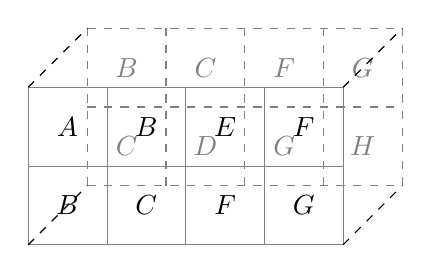
\begin{tikzpicture}
			\draw[step=1cm,gray,very thin] (0,0,0) grid (4,-2,0);
			\draw (0.5,-0.5) node {$A$};
			\draw (1.5,-0.5) node {$B$};
			\draw (0.5,-1.5) node {$B$};
			\draw (1.5,-1.5) node {$C$};

			\draw (2.5,-0.5) node {$E$};
			\draw (3.5,-0.5) node {$F$};
			\draw (2.5,-1.5) node {$F$};
			\draw (3.5,-1.5) node {$G$};

			\begin{scope}[shift={(0.75,0.75,0)}]
				\draw[step=1cm,gray,dashed] (0,0,0) grid (4,-2,0);
				\draw[gray] (0.5,-0.5) node {$B$};
				\draw[gray] (1.5,-0.5) node {$C$};
				\draw[gray] (0.5,-1.5) node {$C$};
				\draw[gray] (1.5,-1.5) node {$D$};

				\draw[gray] (2.5,-0.5) node {$F$};
				\draw[gray] (3.5,-0.5) node {$G$};
				\draw[gray] (2.5,-1.5) node {$G$};
				\draw[gray] (3.5,-1.5) node {$H$};
			\end{scope}

			\draw[dashed] (0,0,0) -- (0.75, 0.75,0);
			\draw[dashed] (4,0,0) -- (4.75, 0.75,0);
			\draw[dashed] (0,-2,0) -- (0.75,-1.25,0);
			\draw[dashed] (4,-2,0) -- (4.75,-1.25,0);
		\end{tikzpicture}

		\vspace{5mm}

		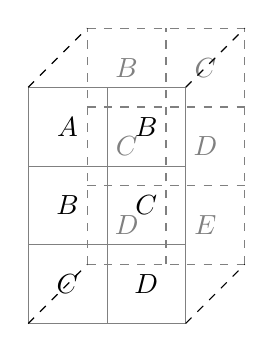
\begin{tikzpicture}
			\draw[step=1cm,gray,very thin] (0,0,0) grid (2,-3,0);
			\draw (0.5,-0.5) node {$A$};
			\draw (1.5,-0.5) node {$B$};
			\draw (0.5,-1.5) node {$B$};
			\draw (1.5,-1.5) node {$C$};
			\draw (0.5,-2.5) node {$C$};
			\draw (1.5,-2.5) node {$D$};

			\begin{scope}[shift={(0.75,0.75,0)}]
				\draw[step=1cm,gray,dashed] (0,0,0) grid (2,-3,0);
				\draw[gray] (0.5,-0.5) node {$B$};
				\draw[gray] (1.5,-0.5) node {$C$};
				\draw[gray] (0.5,-1.5) node {$C$};
				\draw[gray] (1.5,-1.5) node {$D$};
				\draw[gray] (0.5,-2.5) node {$D$};
				\draw[gray] (1.5,-2.5) node {$E$};
			\end{scope}

			\draw[dashed] (0,0,0) -- (0.75, 0.75,0);
			\draw[dashed] (2,0,0) -- (2.75, 0.75,0);
			\draw[dashed] (0,-3,0) -- (0.75,-2.25,0);
			\draw[dashed] (2,-3,0) -- (2.75,-2.25,0);
		\end{tikzpicture}
		\hspace{5mm}
		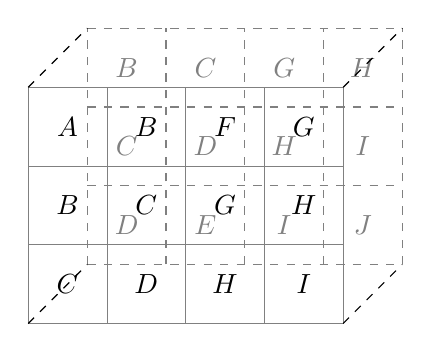
\begin{tikzpicture}
			\draw[step=1cm,gray,very thin] (0,0,0) grid (4,-3,0);
			\draw (0.5,-0.5) node {$A$};
			\draw (1.5,-0.5) node {$B$};
			\draw (0.5,-1.5) node {$B$};
			\draw (1.5,-1.5) node {$C$};
			\draw (0.5,-2.5) node {$C$};
			\draw (1.5,-2.5) node {$D$};

			\draw (2.5,-0.5) node {$F$};
			\draw (3.5,-0.5) node {$G$};
			\draw (2.5,-1.5) node {$G$};
			\draw (3.5,-1.5) node {$H$};
			\draw (2.5,-2.5) node {$H$};
			\draw (3.5,-2.5) node {$I$};

			\begin{scope}[shift={(0.75,0.75,0)}]
				\draw[step=1cm,gray,dashed] (0,0,0) grid (4,-3,0);
				\draw[gray] (0.5,-0.5) node {$B$};
				\draw[gray] (1.5,-0.5) node {$C$};
				\draw[gray] (0.5,-1.5) node {$C$};
				\draw[gray] (1.5,-1.5) node {$D$};
				\draw[gray] (0.5,-2.5) node {$D$};
				\draw[gray] (1.5,-2.5) node {$E$};


				\draw[gray] (2.5,-0.5) node {$G$};
				\draw[gray] (3.5,-0.5) node {$H$};
				\draw[gray] (2.5,-1.5) node {$H$};
				\draw[gray] (3.5,-1.5) node {$I$};
				\draw[gray] (2.5,-2.5) node {$I$};
				\draw[gray] (3.5,-2.5) node {$J$};
			\end{scope}

			\draw[dashed] (0,0,0) -- (0.75, 0.75,0);
			\draw[dashed] (4,0,0) -- (4.75, 0.75,0);
			\draw[dashed] (0,-3,0) -- (0.75,-2.25,0);
			\draw[dashed] (4,-3,0) -- (4.75,-2.25,0);
		\end{tikzpicture}

		\caption{\textit{Top Left:} A cubic curve encoded in a $(2,2,2)$ sized texture, decoded with a single trilinear texture sample. \textit{Top Right:}  Two piecewise cubic curves encoded in a $(4,2,2)$ sized texture, decoded with a single trilinear texture sample.  \textit{Bottom Left:} A Quartic curve encoded in a $(2,3,2)$ sized texture, decoded with two trilinear texture samples. \textit{Bottom Right:} Two piecewise quartic curves encoded in a $(4,3,2)$ sized texture, decoded with two trilinear texture samples.}	
		\label{fig:texlayeout1d}
	\end{figure}	

\end{document}